\documentclass{article}

% content/resources/templates/preamble.tex
\usepackage[margin=0.6in]{geometry}
\author{Milav Dabgar}
\usepackage{amsmath,amssymb,amsthm}
\usepackage{booktabs}
\usepackage{multirow}
\usepackage{xcolor}
\usepackage{tcolorbox}
\tcbuselibrary{breakable,skins}
\usepackage[colorlinks=true,linkcolor=blue]{hyperref}
\usepackage{titlesec}
\usepackage{enumitem}
\usepackage{tikz}
\usepackage{pgfplots}
\usepackage{circuitikz}
\usepackage[version=4]{mhchem}
\usepackage{longtable}
\usepackage{array}
\usepackage{float}
\usepackage{caption}
\usepackage{listings}

\lstset{
  basicstyle=\small\ttfamily,
  breaklines=true,
  breakatwhitespace=false,
  postbreak=\mbox{\textcolor{red}{$\hookrightarrow$}\space},
  float=false,
  numbers=left,
  numberstyle=\tiny\color{gray},
  numbersep=10pt,
  xleftmargin=2em,
  keywordstyle=\color{blue},
  commentstyle=\color{green!60!black},
  stringstyle=\color{purple},
  backgroundcolor=\color{gray!5},
  showstringspaces=false,
  tabsize=2,
  captionpos=b,
  keepspaces=true,
  columns=flexible
}

\pgfplotsset{compat=1.18}
\usetikzlibrary{shapes,arrows,positioning,calc,patterns,decorations.pathmorphing,decorations.markings,arrows.meta}

% Color scheme
\definecolor{headcolor}{RGB}{0,102,204}
\definecolor{keycolor}{RGB}{220,20,60}
\definecolor{solutioncolor}{RGB}{34,139,34}
\definecolor{mnemoniccolor}{RGB}{148,0,211}
\definecolor{codecolor}{RGB}{0,0,100}

% Spacing
\setlength{\parskip}{3pt}
\setlist[itemize]{nosep}
\setlist[enumerate]{nosep}

% Title formatting
\titleformat{\section}{\Large\bfseries\color{headcolor}}{\thesection}{1em}{}
\titleformat{\subsection}{\large\bfseries\color{headcolor}}{\thesubsection}{1em}{}

% Pandoc tightlist compatibility
\providecommand{\tightlist}{%
  \setlength{\itemsep}{0pt}\setlength{\parskip}{0pt}}

% Pandoc longtable compatibility
\newcounter{none}
\def\thenone{}


% content/resources/templates/english-boxes.tex

% Custom environments
\newtcolorbox{solutionbox}{
 breakable,
 enhanced,
 colback=solutioncolor!5!white,
 colframe=solutioncolor!75!black,
 fonttitle=\bfseries,
 title=Solution
}

\newtcolorbox{solutionboxnobreak}{
 colback=solutioncolor!5!white,
 colframe=solutioncolor!75!black,
 fonttitle=\bfseries,
 title=Solution
}

\newtcolorbox{keyformula}{
 breakable,
 enhanced,
 colback=keycolor!5!white,
 colframe=keycolor!75!black,
 fonttitle=\bfseries,
 title=Key Formula
}

\newtcolorbox{mnemonicboxenv}{
 breakable,
 enhanced,
 colback=mnemoniccolor!5!white,
 colframe=mnemoniccolor!75!black,
 fonttitle=\bfseries,
 title=Mnemonic
}

\newcommand{\mnemonicbox}[1]{%
  \begin{mnemonicboxenv}
    #1
  \end{mnemonicboxenv}
}


% Custom commands for GTU solutions
% This file defines semantic commands for consistent formatting

% Question command with automatic formatting
\newcommand{\question}[2]{%
  \section*{Question #1}%
  \textbf{#2}%
}

% OR question variant
\newcommand{\questionor}[2]{%
  \section*{Question #1 OR}%
  \textbf{#2}%
}

% Proper table environment with caption
\newenvironment{answertable}[1]{%
  \begin{table}[htbp]
  \centering
  \caption{#1}
}{%
  \end{table}
}

% Proper figure environment for diagrams
\newenvironment{answerdiagram}[1]{%
  \begin{figure}[htbp]
  \centering
  \caption{#1}
}{%
  \end{figure}
}

% Semantic markup for key terms
\newcommand{\keyword}[1]{\textbf{#1}}
\newcommand{\code}[1]{\texttt{#1}}
\newcommand{\classname}[1]{\texttt{#1}}
\newcommand{\methodname}[1]{\texttt{#1}}

% Proper quotation marks
\newcommand{\mnemonic}[1]{``#1''}


\title{Microwave and Radar Communication (4351103) - Winter 2024 Solution}
\date{November 27, 2024}

\begin{document}
\maketitle

\questionmarks{1(a)}{3}{Give comparison between transmission line and waveguide.}

\begin{solutionbox}
\textbf{Comparison:}

\begin{tabulary}{\linewidth}{|L|L|L|}
\hline
\textbf{Parameter} & \textbf{Transmission Line} & \textbf{Waveguide} \\ \hline
\keyword{Frequency Range} & Low to medium frequencies & High frequencies (above 1 GHz) \\ \hline
\keyword{Structure} & Two or more conductors & Single hollow conductor \\ \hline
\keyword{Propagation Mode} & TEM mode & TE and TM modes \\ \hline
\keyword{Power Handling} & Limited power capacity & High power handling capability \\ \hline
\keyword{Losses} & Higher losses at high frequencies & Lower losses at microwave frequencies \\ \hline
\end{tabulary}
\end{solutionbox}

\begin{mnemonicbox}
\mnemonic{"WAVES Travel Better" (Waveguides - Advanced Versions Enabling Superior Transmission)}
\end{mnemonicbox}

\questionmarks{1(b)}{4}{Define the following terms: (1) Lossless Line (2) VSWR (3) STUB (4) Reflection coefficient}

\begin{solutionbox}
\textbf{Definitions:}

\begin{itemize}
    \item \textbf{Lossless Line}: A transmission line with zero resistance and conductance, having no power loss during signal transmission.
    \item \textbf{VSWR (Voltage Standing Wave Ratio)}: Ratio of maximum voltage to minimum voltage on a transmission line, indicating impedance mismatch.
    \item \textbf{STUB}: Short length of transmission line connected to main line for impedance matching purposes.
    \item \textbf{Reflection Coefficient}: Ratio of reflected wave amplitude to incident wave amplitude at any point on transmission line.
\end{itemize}
\end{solutionbox}

\begin{mnemonicbox}
\mnemonic{"Light Volumes Stay Reflected" (Lossless-VSWR-Stub-Reflection)}
\end{mnemonicbox}

\questionmarks{1(c)}{7}{Explain isolator and circulator with the help of sketch.}

\begin{solutionbox}
\textbf{Isolator:}
\begin{enumerate}
    \item \textbf{Function}: Allows signal flow in one direction only.
    \item \textbf{Construction}: Uses ferrite material with magnetic bias.
    \item \textbf{Applications}: Protects sources from reflections.
\end{enumerate}

\begin{answerdiagram}{Isolator Symbol}
\begin{tikzpicture}[auto, node distance=2cm]
    \node [gtu block] (iso) {Isolator};
    \node [gtu input, left=of iso] (p1) {Port 1};
    \node [gtu output, right=of iso] (p2) {Port 2};
    
    \draw [gtu arrow] (p1) -- (iso);
    \draw [gtu arrow] (iso) -- (p2);
    
    % Reflection blocked
    \draw [->, red, dashed, bend left] (p2) to node[above] {X} (iso);
\end{tikzpicture}
\end{answerdiagram}

\textbf{Circulator:}
\begin{enumerate}
    \item \textbf{Function}: Routes signals in circular pattern between three or four ports.
    \item \textbf{Construction}: Y-junction with ferrite material.
    \item \textbf{Applications}: Duplexers in radar systems.
\end{enumerate}

\begin{answerdiagram}{Circulator Symbol}
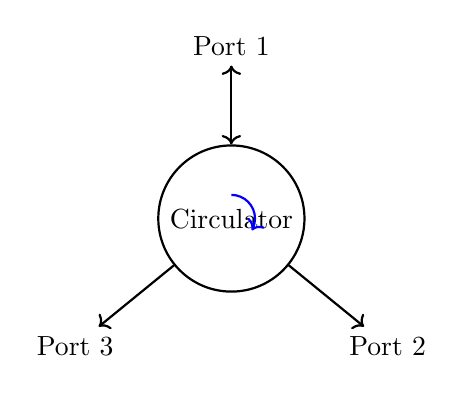
\begin{tikzpicture}
    \node [draw, circle, minimum size=1.5cm, thick] (c) {Circulator};
    \node [above=1cm of c] (p1) {Port 1};
    \node [below right=1cm of c] (p2) {Port 2};
    \node [below left=1cm of c] (p3) {Port 3};
    
    \draw [->, thick] (p1) -- (c);
    \draw [->, thick] (c) -- (p2);
    \draw [->, thick] (c) -- (p3);
    \draw [->, thick] (c) -- (p1);
    
    \draw [->, thick, blue] (0,0.3) arc (90:-30:0.3);
\end{tikzpicture}
\end{answerdiagram}
\end{solutionbox}

\begin{mnemonicbox}
\mnemonic{"Isolated Circuits Flow Forward" (Isolator-Circulator-Forward-Flow)}
\end{mnemonicbox}

\orquestionmarks{1(c)}{7}{What is dominant mode in a waveguide? What will be the cutoff wavelength for dominant mode, in a rectangular waveguide whose breadth is 10 cm? For a 2.5 GHz signal propagated through it calculate guide wavelength, group velocity and phase velocity and Z₀.}

\begin{solutionbox}
\textbf{Dominant Mode:} Lowest order mode that can propagate in a waveguide. For rectangular waveguide, it's TE$_{10}$ mode.

\textbf{Given Data:}
\begin{itemize}
    \item Breadth (a) = 10 cm = 0.1 m
    \item Frequency (f) = 2.5 GHz = $2.5 \times 10^9$ Hz
    \item c = $3 \times 10^8$ m/s
\end{itemize}

\textbf{Calculations:}
\begin{tabulary}{\linewidth}{|L|L|L|}
\hline
\textbf{Parameter} & \textbf{Formula} & \textbf{Value} \\ \hline
Cutoff Wavelength & $\lambda_c = 2a$ & $\lambda_c = 2 \times 0.1 = 0.2$ m \\ \hline
Free Space Wavelength & $\lambda_0 = c/f$ & $\lambda_0 = 0.12$ m \\ \hline
Guide Wavelength & $\lambda_g = \frac{\lambda_0}{\sqrt{1-(\lambda_0/\lambda_c)^2}}$ & $\lambda_g = 0.133$ m \\ \hline
Group Velocity & $v_g = c\sqrt{1-(\lambda_0/\lambda_c)^2}$ & $v_g = 2.7 \times 10^8$ m/s \\ \hline
Phase Velocity & $v_p = \frac{c}{\sqrt{1-(\lambda_0/\lambda_c)^2}}$ & $v_p = 3.33 \times 10^8$ m/s \\ \hline
\end{tabulary}
\end{solutionbox}

\begin{mnemonicbox}
\mnemonic{"Dominant Modes Calculate Guide Parameters"}
\end{mnemonicbox}

\questionmarks{2(a)}{3}{What is single stub impedance matching, and how does it work?}

\begin{solutionbox}
\textbf{Single Stub Matching:} Technique using one short-circuited or open-circuited stub connected in parallel to transmission line for impedance matching.

\textbf{Working Principle:}
\begin{itemize}
    \item \textbf{Stub acts as reactive element} (inductive or capacitive).
    \item \textbf{Cancels reactive component} of load impedance.
    \item \textbf{Transforms impedance} to characteristic impedance.
\end{itemize}
\end{solutionbox}

\begin{mnemonicbox}
\mnemonic{"Single Stubs Transform Reactance" (Single-Stub-Transform-Reactive)}
\end{mnemonicbox}

\questionmarks{2(b)}{4}{Differentiate between rectangular and circular waveguide any three points.}

\begin{solutionbox}
\textbf{Comparison:}

\begin{tabulary}{\linewidth}{|L|L|L|}
\hline
\textbf{Parameter} & \textbf{Rectangular Waveguide} & \textbf{Circular Waveguide} \\ \hline
\keyword{Cross-section} & Rectangular shape & Circular shape \\ \hline
\keyword{Dominant Mode} & TE$_{10}$ mode & TE$_{11}$ mode \\ \hline
\keyword{Field Pattern} & Simple field distribution & Complex field distribution \\ \hline
\keyword{Manufacturing} & Easy to manufacture & Difficult to manufacture \\ \hline
\end{tabulary}
\end{solutionbox}

\begin{mnemonicbox}
\mnemonic{"Rectangles Dominate Ten" vs "Circles Dominate Eleven"}
\end{mnemonicbox}

\questionmarks{2(c)}{7}{Explain the construction and working of Hybrid Ring with diagram.}

\begin{solutionbox}
\textbf{Construction:}
\begin{itemize}
    \item \textbf{Ring structure} with four ports.
    \item \textbf{Circumference} = 1.5$\lambda$ (one and half wavelengths).
    \item \textbf{Adjacent ports} separated by $\lambda/4$.
    \item \textbf{Opposite ports} separated by 3$\lambda/4$.
\end{itemize}

\begin{answerdiagram}{Hybrid Ring (Rat-Race Coupler)}
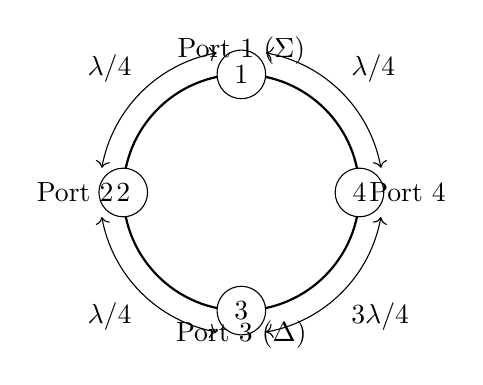
\begin{tikzpicture}[scale=1.5]
    \draw [thick] (0,0) circle (1cm);
    
    \node [draw, circle, fill=white] at (90:1cm)  (p1) {1};
    \node [draw, circle, fill=white] at (180:1cm) (p2) {2};
    \node [draw, circle, fill=white] at (270:1cm) (p3) {3};
    \node [draw, circle, fill=white] at (0:1cm)   (p4) {4};
    
    \node [above] at (p1) {Port 1 ($\Sigma$)};
    \node [left] at (p2) {Port 2};
    \node [below] at (p3) {Port 3 ($\Delta$)};
    \node [right] at (p4) {Port 4};
    
    \draw [<->] (10:1.2) arc (10:80:1.2) node [midway, above right] {$\lambda/4$};
    \draw [<->] (100:1.2) arc (100:170:1.2) node [midway, above left] {$\lambda/4$};
    \draw [<->] (190:1.2) arc (190:260:1.2) node [midway, below left] {$\lambda/4$};
    \draw [<->] (280:1.2) arc (280:350:1.2) node [midway, below right] {$3\lambda/4$};
\end{tikzpicture}
\end{answerdiagram}

\textbf{Working:}
\begin{itemize}
    \item \textbf{Power division}: Input at one port divides equally between two adjacent ports.
    \item \textbf{Isolation}: Opposite port receives no power.
    \item \textbf{Phase relationship}: 180$^\circ$ phase difference between output ports.
\end{itemize}

\textbf{Applications:} Balanced mixers, Power combiners/dividers, Antenna feeds.
\end{solutionbox}

\begin{mnemonicbox}
\mnemonic{"Hybrid Rings Divide Power Equally"}
\end{mnemonicbox}

\orquestionmarks{2(a)}{3}{What is Microwave? List out any four applications of microwave.}

\begin{solutionbox}
\textbf{Microwave:} Electromagnetic waves with frequency range from 1 GHz to 300 GHz.

\textbf{Applications:}
\begin{enumerate}
    \item \textbf{Radar systems}: for detection and ranging.
    \item \textbf{Satellite communication}: for long-distance transmission.
    \item \textbf{Microwave ovens}: for heating food.
    \item \textbf{Mobile communication}: (cellular networks).
\end{enumerate}
\end{solutionbox}

\begin{mnemonicbox}
\mnemonic{"Microwaves Reach Space Mobile" (Microwave-Radar-Satellite-Mobile)}
\end{mnemonicbox}

\orquestionmarks{2(b)}{4}{Write short note on cavity resonator.}

\begin{solutionbox}
\textbf{Cavity Resonator:} Closed metallic structure that confines electromagnetic energy at specific resonant frequencies.

\textbf{Construction:}
\begin{itemize}
    \item \textbf{Metallic enclosure} of specific dimensions.
    \item \textbf{High Q factor} (low losses).
    \item \textbf{Resonant frequency} depends on cavity dimensions.
\end{itemize}

\textbf{Types:} Rectangular cavity, Cylindrical cavity, Spherical cavity.

\textbf{Applications:} Frequency meters, Oscillator circuits, Filter circuits.
\end{solutionbox}

\begin{mnemonicbox}
\mnemonic{"Cavities Resonate High Quality" (Cavity-Resonant-High-Q)}
\end{mnemonicbox}

\orquestionmarks{2(c)}{7}{Explain MAGIC TEE with the help of sketch and how it works as an isolator?}

\begin{solutionbox}
\textbf{Magic Tee Construction:}
\begin{itemize}
    \item \textbf{E-plane Tee} and \textbf{H-plane Tee} combined.
    \item \textbf{Four ports}: E-arm, H-arm, and two side arms (Collinear arms).
    \item \textbf{E-arm} perpendicular to H-arm.
\end{itemize}

\begin{answerdiagram}{Magic Tee}
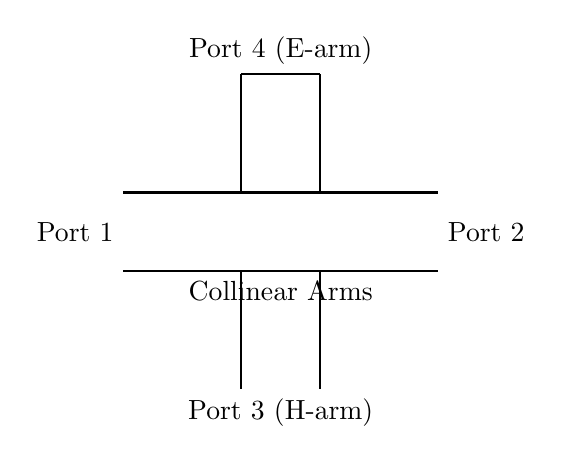
\begin{tikzpicture}[scale=1]
    % H-arm
    \draw [thick] (-2,0) -- (2,0);
    \draw [thick] (-2,1) -- (2,1);
    \node [left] at (-2,0.5) {Port 1};
    \node [right] at (2,0.5) {Port 2};
    \node [below] at (0,0) {Collinear Arms};

    % E-arm
    \draw [thick] (-0.5,1) -- (-0.5,2.5);
    \draw [thick] (0.5,1) -- (0.5,2.5);
    \draw [thick] (-0.5,2.5) -- (0.5,2.5);
    \node [above] at (0,2.5) {Port 4 (E-arm)};

    % H-arm vertical part
    \draw [thick] (-0.5,0) -- (-0.5,-1.5);
    \draw [thick] (0.5,0) -- (0.5,-1.5);
    \node [below] at (0,-1.5) {Port 3 (H-arm)};
\end{tikzpicture}
\end{answerdiagram}

\textbf{Working as Isolator:}
\begin{itemize}
    \item \textbf{Signal at E-arm}: Divides equally between side arms (in-phase).
    \item \textbf{Signal at H-arm}: Divides equally between side arms (out-of-phase).
    \item \textbf{Isolation}: Between E-arm and H-arm.
    \item \textbf{No coupling}: Between perpendicular arms.
\end{itemize}

\textbf{Properties:} Matched at all ports, Reciprocal device, Power division and isolation.
\end{solutionbox}

\begin{mnemonicbox}
\mnemonic{"Magic Isolates Perpendicular Arms"}
\end{mnemonicbox}

\questionmarks{3(a)}{3}{Describe the working principle of MASER.}

\begin{solutionbox}
\textbf{MASER (Microwave Amplification by Stimulated Emission of Radiation):}
\begin{enumerate}
    \item \keyword{Population Inversion}: Created in active medium.
    \item \keyword{Stimulated Emission}: Produces coherent microwaves.
    \item \keyword{Amplification}: Occurs through energy level transitions.
\end{enumerate}

\textbf{Working Principle:}
Atoms excited to higher energy levels -> Stimulated photons trigger emission -> Coherent amplification of microwave signals.
\end{solutionbox}

\begin{mnemonicbox}
\mnemonic{"Microwaves Amplify Stimulated Emission Radiation"}
\end{mnemonicbox}

\questionmarks{3(b)}{4}{List four microwave diodes and explain any one.}

\begin{solutionbox}
\textbf{Four Microwave Diodes:}
1. GUNN Diode, 2. IMPATT Diode, 3. TRAPATT Diode, 4. PIN Diode.

\textbf{GUNN Diode:}
\begin{itemize}
    \item \textbf{Principle}: Transferred electron effect in GaAs.
    \item \textbf{Construction}: N-type GaAs with ohmic contacts.
    \item \textbf{Operation}: Negative resistance at microwave frequencies.
    \item \textbf{Applications}: Oscillators, amplifiers.
\end{itemize}

\begin{answerdiagram}{Gunn Diode I-V Characteristics}
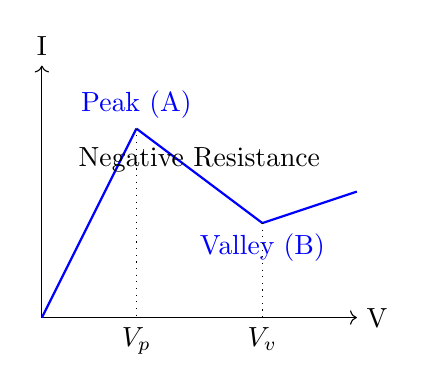
\begin{tikzpicture}[scale=0.8]
    \draw[->] (0,0) -- (5,0) node[right] {V};
    \draw[->] (0,0) -- (0,4) node[above] {I};
    
    \draw[thick, blue] (0,0) -- (1.5,3) node[above] {Peak (A)};
    \draw[thick, blue] (1.5,3) -- (3.5,1.5) node[below] {Valley (B)};
    \draw[thick, blue] (3.5,1.5) -- (5,2);
    
    \node at (2.5, 2.5) {Negative Resistance};
    \draw[dotted] (1.5,3) -- (1.5,0) node[below] {$V_p$};
    \draw[dotted] (3.5,1.5) -- (3.5,0) node[below] {$V_v$};
\end{tikzpicture}
\end{answerdiagram}
\end{solutionbox}

\begin{mnemonicbox}
\mnemonic{"GUNN Generates Negative Resistance"}
\end{mnemonicbox}

\questionmarks{3(c)}{7}{Write a detailed explanation of the Magnetron Oscillator, covering its construction, working principle, and applications?}

\begin{solutionbox}
\textbf{Construction:}
\begin{itemize}
    \item \textbf{Cylindrical cathode} at center.
    \item \textbf{Anode with resonant cavities} surrounding cathode.
    \item \textbf{Strong magnetic field} perpendicular to electric field.
    \item \textbf{Output coupling} through waveguide.
\end{itemize}

\begin{answerdiagram}{Magnetron Construction}
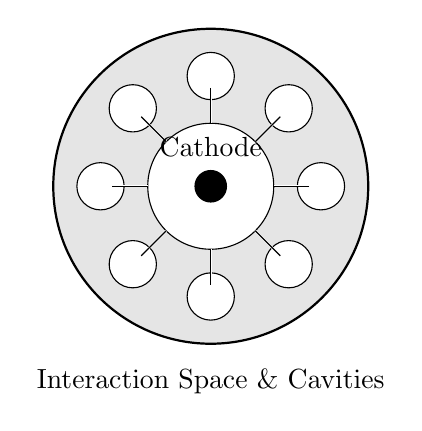
\begin{tikzpicture}
    % Anode Block
    \draw[thick, fill=gray!20] (0,0) circle (2);
    \draw[fill=white] (0,0) circle (0.8);
    
    % Cavities
    \foreach \a in {0,45,...,315} {
        \draw[fill=white] (\a:1.4) circle (0.3);
        \draw[white, thick] (\a:1.4) -- (\a:0.8);
        \draw (\a:1.25) -- (\a:0.8);
    }
    
    % Cathode
    \draw[fill=black] (0,0) circle (0.2);
    \node at (0,0.5) {Cathode};
    
    \node[below] at (0,-2.2) {Interaction Space \& Cavities};
\end{tikzpicture}
\end{answerdiagram}

\textbf{Working Principle:}
\begin{itemize}
    \item Electrons emitted from heated cathode.
    \item \keyword{Cycloid motion} due to crossed E and B fields.
    \item \keyword{Bunching effect} creates electron clouds.
    \item Energy transfer from electrons to RF field.
    \item Oscillation at cavity resonant frequency.
\end{itemize}

\textbf{Applications:} Radar transmitters, Microwave ovens, Industrial heating.
\end{solutionbox}

\begin{mnemonicbox}
\mnemonic{"Magnetrons Make Microwave Oscillations"}
\end{mnemonicbox}

\orquestionmarks{3(a)}{3}{Describe the working of RUBY MASER.}

\begin{solutionbox}
\textbf{Ruby MASER Working:}
\begin{itemize}
    \item \textbf{Ruby crystal} (Al$_2$O$_3$ with Cr$^{3+}$ ions) as active medium.
    \item \textbf{Three energy levels} in chromium ions.
    \item \textbf{Pump frequency} creates population inversion.
    \item \textbf{Signal amplification} at 2.9 GHz.
\end{itemize}

\textbf{Process:} Optical pumping excites electrons to higher level -> Stimulated emission produces coherent microwaves -> Low noise amplification achieved.
\end{solutionbox}

\begin{mnemonicbox}
\mnemonic{"Ruby Radiates Amplified Microwaves"}
\end{mnemonicbox}

\orquestionmarks{3(b)}{4}{Draw and explain the VI characteristic of Gun diode}

\begin{solutionbox}
\begin{answerdiagram}{Gunn Diode I-V Characteristics}
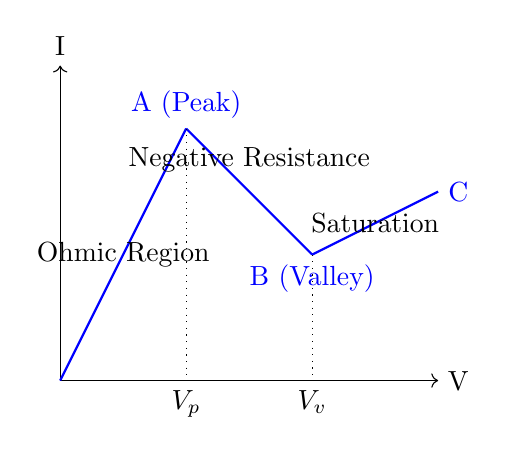
\begin{tikzpicture}[scale=0.8]
    \draw[->] (0,0) -- (6,0) node[right] {V};
    \draw[->] (0,0) -- (0,5) node[above] {I};
    
    \draw[thick, blue] (0,0) -- (2,4) node[above] {A (Peak)};
    \draw[thick, blue] (2,4) -- (4,2) node[below] {B (Valley)};
    \draw[thick, blue] (4,2) -- (6,3) node[right] {C};
    
    \node at (1, 2) {Ohmic Region};
    \node at (3, 3.5) {Negative Resistance};
    \node at (5, 2.5) {Saturation};
    
    \draw[dotted] (2,4) -- (2,0) node[below] {$V_p$};
    \draw[dotted] (4,2) -- (4,0) node[below] {$V_v$};
\end{tikzpicture}
\end{answerdiagram}

\textbf{Explanation:}
\begin{itemize}
    \item \textbf{Region OA}: Ohmic region (positive resistance).
    \item \textbf{Region AB}: Negative resistance region.
    \item \textbf{Region BC}: Valley current region.
    \item \textbf{Region CD}: Saturation region.
\end{itemize}

\textbf{Key Points:}
\begin{itemize}
    \item \textbf{Peak voltage}: Maximum voltage before negative resistance.
    \item \textbf{Valley current}: Minimum current in negative resistance region.
    \item \textbf{Negative resistance}: Current decreases with increasing voltage.
\end{itemize}
\end{solutionbox}

\begin{mnemonicbox}
\mnemonic{"Valley Peak Negative Resistance"}
\end{mnemonicbox}

\orquestionmarks{3(c)}{7}{Explain "frequency measurement method" as well as "attenuation measurement method" at microwave frequency.}

\begin{solutionbox}
\textbf{Frequency Measurement Methods:}
\begin{tabulary}{\linewidth}{|L|L|L|}
\hline
\textbf{Method} & \textbf{Principle} & \textbf{Accuracy} \\ \hline
Cavity Wavemeter & Resonant cavity tuning & High \\ \hline
Direct Reading Meter & Frequency counter & Very High \\ \hline
Heterodyne Method & Beat frequency technique & Medium \\ \hline
\end{tabulary}

\textbf{Attenuation Measurement Methods:}
\begin{tabulary}{\linewidth}{|L|L|L|}
\hline
\textbf{Method} & \textbf{Description} & \textbf{Application} \\ \hline
Substitution Method & Replace attenuator with calibrated attenuator & Precision measurement \\ \hline
Power Ratio Method & Compare input and output power & General purpose \\ \hline
RF Bridge Method & Balance bridge circuit & Laboratory use \\ \hline
\end{tabulary}

\textbf{Setup for Measurement:}
\begin{itemize}
    \item \textbf{Signal generator} provides test signal.
    \item \textbf{Calibrated attenuator} for reference.
    \item \textbf{Power meter} measures signal levels.
    \item \textbf{VSWR meter} monitors impedance matching.
\end{itemize}
\end{solutionbox}

\begin{mnemonicbox}
\mnemonic{"Frequency Attenuation Measured Precisely"}
\end{mnemonicbox}

\questionmarks{4(a)}{3}{Explain working of P-i-N diode.}

\begin{solutionbox}
\textbf{Structure:} P-type region (heavily doped), Intrinsic region (undoped, high resistance), N-type region (heavily doped).

\textbf{Working:}
\begin{itemize}
    \item \textbf{Forward bias}: Low resistance, acts as conductor.
    \item \textbf{Reverse bias}: High resistance, acts as insulator.
    \item \textbf{RF switching}: Fast switching due to charge storage.
\end{itemize}

\textbf{Applications:} RF switches, Attenuators, Phase shifters.
\end{solutionbox}

\begin{mnemonicbox}
\mnemonic{"PIN Provides Instant Switching"}
\end{mnemonicbox}

\questionmarks{4(b)}{4}{Explain $\pi$ mode oscillations for magnetron.}

\begin{solutionbox}
\textbf{$\pi$ Mode Oscillation:}
\begin{itemize}
    \item \textbf{Adjacent cavities} oscillate 180$^\circ$ out of phase.
    \item \textbf{Electron bunching} synchronized with RF field.
    \item \textbf{Maximum power transfer} from electrons to RF.
    \item \textbf{Stable oscillation} at designed frequency.
\end{itemize}

\textbf{Mode Chart:}
\begin{center}
Cavity: 1 --- 2 --- 3 --- 4 --- 5 --- 6 --- 7 --- 8 \\
Phase: 0 --- $\pi$ --- 0 --- $\pi$ --- 0 --- $\pi$ --- 0 --- $\pi$
\end{center}
\end{solutionbox}

\begin{mnemonicbox}
\mnemonic{"Pi Mode Produces Maximum Power"}
\end{mnemonicbox}

\questionmarks{4(c)}{7}{Explain the construction and working of two cavity klystron amplifiers with necessary diagram.}

\begin{solutionbox}
\begin{answerdiagram}{Two Cavity Klystron}
\begin{tikzpicture}[auto, node distance=1.5cm]
    \node [gtu start] (gun) {Electron Gun};
    \node [gtu block, right=of gun] (buncher) {Buncher};
    \node [gtu block, right=of buncher, minimum width=2.5cm] (drift) {Drift Space};
    \node [gtu block, right=of drift] (catcher) {Catcher};
    \node [gtu stop, right=of catcher] (coll) {Collector};
    
    \draw [gtu arrow] (gun) -- (buncher);
    \draw [gtu arrow] (buncher) -- (drift);
    \draw [gtu arrow] (drift) -- (catcher);
    \draw [gtu arrow] (catcher) -- (coll);
    
    \draw [<-] (buncher.south) -- +(0,-0.5) node[below] {RF In};
    \draw [->] (catcher.south) -- +(0,-0.5) node[below] {RF Out};
\end{tikzpicture}
\end{answerdiagram}

\textbf{Construction:}
\begin{itemize}
    \item \textbf{Electron gun} produces electron beam.
    \item \textbf{Input cavity} (buncher) modulates electron beam.
    \item \textbf{Drift space} allows velocity modulation.
    \item \textbf{Output cavity} (catcher) extracts RF energy.
    \item \textbf{Collector} collects spent electrons.
\end{itemize}

\textbf{Working Principle:}
Velocity modulation in input cavity -> Electron bunching in drift space -> Density modulation creates current variation -> Energy extraction in output cavity -> Amplification.
\end{solutionbox}

\begin{mnemonicbox}
\mnemonic{"Klystrons Amplify Through Bunching"}
\end{mnemonicbox}

\orquestionmarks{4(a)}{3}{Explain parametric amplifier.}

\begin{solutionbox}
\textbf{Parametric Amplifier:}
\begin{itemize}
    \item \textbf{Variable reactance} device using varactor diode.
    \item \textbf{Pump frequency} modulates diode capacitance.
    \item \textbf{Energy transfer} from pump to signal.
    \item \textbf{Low noise amplification} achieved.
\end{itemize}

\textbf{Working:}
Pump power varies diode reactance -> Signal mixing produces sum and difference frequencies -> Idler frequency $f_p = f_s + f_i$ -> Power gain through nonlinear mixing.
\end{solutionbox}

\begin{mnemonicbox}
\mnemonic{"Parametric Amplifiers Pump Low Noise"}
\end{mnemonicbox}

\orquestionmarks{4(b)}{4}{Draw and explain schematic diagram of travelling wave tube with necessary notation}

\begin{solutionbox}
\begin{answerdiagram}{Traveling Wave Tube}
\begin{tikzpicture}[auto, node distance=1.5cm]
    \node [gtu start] (gun) {Electron Gun};
    \node [gtu block, right=of gun, minimum width=4cm] (helix) {Helix};
    \node [gtu stop, right=of helix] (col) {Collector};
    
    \draw [gtu arrow] (gun) -- (helix);
    \draw [gtu arrow] (helix) -- (col);
    
    \draw [<-] (2, 0.5) -- (2, 1) node[above] {RF In};
    \draw [->] (5, 0.5) -- (5, 1) node[above] {RF Out};
    
    \node [below] at (3.5, -0.5) {Attenuator};
\end{tikzpicture}
\end{answerdiagram}

\textbf{Working:}
\begin{itemize}
    \item \textbf{Electron beam} travels through helix center.
    \item \textbf{RF signal} propagates along helix.
    \item \textbf{Synchronism} between beam and RF wave.
    \item \textbf{Energy transfer} from beam to RF.
    \item \textbf{Continuous amplification} along helix length.
\end{itemize}
\end{solutionbox}

\begin{mnemonicbox}
\mnemonic{"TWT Travels With Waves"}
\end{mnemonicbox}

\orquestionmarks{4(c)}{7}{Explain the working principle of a reflex klystron in detail with suitable diagram.}

\begin{solutionbox}
\begin{answerdiagram}{Reflex Klystron Schematic}
\begin{tikzpicture}[auto, node distance=1.5cm]
    \node [gtu start] (cath) {Cathode};
    \node [gtu block, right=of cath] (cav) {Cavity};
    \node [gtu block, right=of cav] (rep) {Repeller};
    
    \draw [gtu arrow] (cath) -- (cav);
    \draw [gtu arrow] (cav) -- (rep);
    \draw [->, bend right, dashed] (rep) to node[above] {Reflected e$^-$} (cav);
    
    \draw [->] (cav.south) -- +(0,-0.5) node[below] {RF Output};
\end{tikzpicture}
\end{answerdiagram}

\textbf{Working Principle:}
\begin{enumerate}
    \item \textbf{Electrons enter cavity} and get velocity modulated.
    \item \textbf{Electrons drift} toward repeller.
    \item \textbf{Repeller reflects} electrons back to cavity.
    \item \textbf{Transit time} determines bunching phase.
    \item \textbf{Bunched electrons} deliver energy to cavity.
    \item \textbf{Oscillation maintained} through feedback.
\end{enumerate}

\textbf{Applications:} Local oscillators, Frequency meters, Microwave sources.
\end{solutionbox}

\begin{mnemonicbox}
\mnemonic{"Reflex Returns Electron Bunches"}
\end{mnemonicbox}

\questionmarks{5(a)}{3}{"PIN diode acts as a switch and VARACTOR diode acts as a variable capacitor" explain.}

\begin{solutionbox}
\textbf{PIN Diode as Switch:}
\begin{itemize}
    \item \textbf{Forward bias}: Low resistance ($\sim 1\Omega$), switch ON.
    \item \textbf{Reverse bias}: High resistance ($\sim 10k\Omega$), switch OFF.
    \item \textbf{Fast switching} due to charge storage in I-region.
    \item \textbf{RF isolation} in OFF state.
\end{itemize}

\textbf{VARACTOR Diode as Variable Capacitor:}
\begin{itemize}
    \item \textbf{Reverse bias voltage} controls junction capacitance.
    \item \textbf{Capacitance decreases} with increasing reverse voltage ($C \propto V^{-n}$).
    \item \textbf{Voltage-controlled reactance} for tuning circuits.
    \item \textbf{Electronic tuning} without mechanical adjustment.
\end{itemize}
\end{solutionbox}

\begin{mnemonicbox}
\mnemonic{"PIN Switches, VARACTOR Varies"}
\end{mnemonicbox}

\questionmarks{5(b)}{4}{List the display methods used in RADAR and explain any one.}

\begin{solutionbox}
\textbf{RADAR Display Methods:}
1. A-Scope Display, 2. PPI (Plan Position Indicator), 3. B-Scope Display, 4. RHI (Range Height Indicator).

\textbf{PPI Display Explanation:}
\begin{itemize}
    \item \textbf{Circular display} showing target positions.
    \item \textbf{Center represents} radar location.
    \item \textbf{Radial distance} indicates target range.
    \item \textbf{Angular position} shows target bearing.
    \item \textbf{Rotating sweep} synchronized with antenna rotation.
\end{itemize}
Features: Real-time display, Range and bearing info, Multiple target tracking.
\end{solutionbox}

\begin{mnemonicbox}
\mnemonic{"PPI Pictures Position Indicators"}
\end{mnemonicbox}

\questionmarks{5(c)}{7}{What is radar? List out the different types of radar systems? Explain any One of radar in detail?}

\begin{solutionbox}
\textbf{RADAR (Radio Detection And Ranging):} System using radio waves to detect objects and determine their range, velocity, and characteristics.

\textbf{Types of RADAR Systems:}
\begin{tabulary}{\linewidth}{|L|L|L|}
\hline
\textbf{Type} & \textbf{Application} & \textbf{Frequency Band} \\ \hline
Pulse Radar & Air traffic control & L, S, C bands \\ \hline
CW Doppler Radar & Speed measurement & X, K, Ka bands \\ \hline
MTI Radar & Moving target detection & S, C bands \\ \hline
SAR Radar & Ground mapping & L, C, X bands \\ \hline
\end{tabulary}

\textbf{Pulse Radar Detailed Explanation:}

\begin{answerdiagram}{Pulse Radar Block Diagram}
\begin{tikzpicture}[auto, node distance=1.5cm]
    \node [gtu block] (tim) {Timer};
    \node [gtu block, below=of tim] (mod) {Modulator};
    \node [gtu block, right=of mod] (tx) {Transmitter};
    \node [gtu block, right=of tx] (dup) {Duplexer};
    \node [gtu block, right=of dup] (ant) {Antenna};
    \node [gtu block, below=of dup] (rx) {Receiver};
    \node [gtu block, left=of rx] (disp) {Display};
    
    \draw [gtu arrow] (tim) -- (mod);
    \draw [gtu arrow] (mod) -- (tx);
    \draw [gtu arrow] (tx) -- (dup);
    \draw [gtu arrow] (dup) -- (ant);
    \draw [gtu arrow] (ant) -- (dup);
    \draw [gtu arrow] (dup) -- (rx);
    \draw [gtu arrow] (rx) -- (disp);
    \draw [gtu arrow] (tim) -| (disp);
\end{tikzpicture}
\end{answerdiagram}

\textbf{Working:}
\begin{itemize}
    \item \textbf{Transmits short pulses} of RF energy.
    \item \textbf{Receives echoes} from targets.
    \item \textbf{Measures time delay} for range calculation.
    \item \textbf{Processes signals} for display.
\end{itemize}

\textbf{Range Equation:} $R = (c \times t)/2$.
\end{solutionbox}

\orquestionmarks{5(a)}{3}{Describe the operation of TRAPATT diode with diagram.}

\begin{solutionbox}
\textbf{TRAPATT Operation:}
\begin{itemize}
    \item \textbf{TRApped Plasma Avalanche Triggered Transit} diode.
    \item \textbf{High field region} creates avalanche breakdown.
    \item \textbf{Plasma formation} traps charge carriers.
    \item \textbf{Transit time effects} create negative resistance.
    \item \textbf{Oscillation frequency} determined by transit time.
\end{itemize}

\begin{answerdiagram}{TRAPATT Diode Operation}
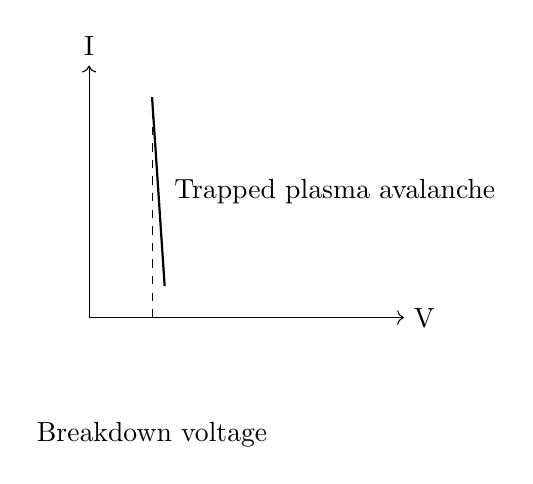
\begin{tikzpicture}[scale=0.8]
    \draw[->] (0,0) -- (5,0) node[right] {V};
    \draw[->] (0,0) -- (0,4) node[above] {I};
    
    \draw[thick] (1,3.5) -- (1.2,0.5);
    \node[right] at (1.2, 2) {Trapped plasma avalanche};
    \draw[dashed] (1,0) -- (1,3.5) node[below, yshift=-4cm] {Breakdown voltage};
\end{tikzpicture}
\end{answerdiagram}

\textbf{Applications:} High power oscillators, Radar transmitters, Communication systems.
\end{solutionbox}

\begin{mnemonicbox}
\mnemonic{"TRAPATT Traps Plasma Avalanche"}
\end{mnemonicbox}

\orquestionmarks{5(b)}{4}{Compare RADAR with SONAR.}

\begin{solutionbox}
\textbf{Comparison:}

\begin{tabulary}{\linewidth}{|L|L|L|}
\hline
\textbf{Parameter} & \textbf{RADAR} & \textbf{SONAR} \\ \hline
\keyword{Wave Type} & Electromagnetic waves & Sound waves \\ \hline
\keyword{Medium} & Air/vacuum & Water/liquid \\ \hline
\keyword{Frequency} & GHz range & kHz range \\ \hline
\keyword{Speed} & $3 \times 10^8$ m/s & 1500 m/s in water \\ \hline
\keyword{Range} & Very long range & Limited by absorption \\ \hline
\keyword{Applications} & Air/space detection & Underwater detection \\ \hline
\end{tabulary}

\textbf{Similarities:} Echo principle for detection, Range measurement using time delay, Doppler effect for velocity measurement.
\end{solutionbox}

\begin{mnemonicbox}
\mnemonic{"RADAR Radiates, SONAR Sounds"}
\end{mnemonicbox}

\orquestionmarks{5(c)}{7}{Obtain the equation for maximum radar range.}

\begin{solutionbox}
\textbf{RADAR Range Equation Derivation:}

1. \textbf{Power Transmitted:} $P_t$

2. \textbf{Power Density at Target:}
   $$P_d = \frac{P_t}{4\pi R^2}$$

3. \textbf{Power Intercepted by Target:}
   $$P_i = P_d \times \sigma = \frac{P_t \times \sigma}{4\pi R^2}$$

4. \textbf{Power Returned to Radar:}
   $$P_r = \frac{P_i}{4\pi R^2} = \frac{P_t \times \sigma}{(4\pi R^2)^2}$$

5. \textbf{Power Received:}
   $$P_r = \frac{P_t \times G^2 \times \lambda^2 \times \sigma}{(4\pi)^3 \times R^4}$$

\textbf{Maximum Range Equation:}
$$R_{max} = \sqrt[4]{\frac{P_t \times G^2 \times \lambda^2 \times \sigma}{(4\pi)^3 \times P_{r_{min}}}}$$

\textbf{Where:}
\begin{itemize}
    \item $P_t$ = Transmitted power
    \item $G$ = Antenna gain
    \item $\lambda$ = Wavelength
    \item $\sigma$ = Radar cross section
    \item $P_{r_{min}}$ = Minimum detectable signal
    \item $R$ = Range
\end{itemize}

\textbf{Factors Affecting Range:} Transmitted power, Antenna gain, Target cross-section, Frequency, Receiver sensitivity.
\end{solutionbox}

\begin{mnemonicbox}
\mnemonic{"Power Gain Lambda Sigma Range"}
\end{mnemonicbox}

\end{document}
